\chapter{Homolog\'ia Persistente}

La homolog\'ia persistente es una herramienta poderosa que es usada para el computo, estudio y codificaci\'on
multiescala de propiedades topol\'ogicas de familias anidadas de complejos simpliciales y espacios
topol\'ogicos. No solo provee algoritmos eficientes para calcular los n\'umeros de Betti de cada complejo
en las familias consideradas, como se requiere para la inferencia homol\'ogica cubierta en la secci\'on
anterior, sino que tambi\'en codifica la evoluci\'on de los grupos de homolog\'ia de los
complejos anidados a trav\'es de las escalas. Ideas y resultados preliminares que culminan en la
teor\'ia de la homolog\'ia persistente pueden ser encontrados desde antes del siglo XXI, en particular
en los trabajos de Barannikov (1994) \cite{Barannikov1994}, Frosini (1992) \cite{Frosini1992},
Robins (1999) \cite{Robins1999}; pero su desarrollo en su forma moderna se concreto en los trabajos
de Edelsbrunner et al. (2002) \cite{Edelsbrunner2002} y Zomorodian y Carlsson (2005)
\cite{Zomorodian2005}.

\section{Filtraciones}

Una filtraci\'on de un complejo simplicial $K$ es una familia anidada de subcomplejos
$\cpar{K_{r}}_{r\in t}$, donde $T\subseteq\mathbb{R}$, tal que para cualquier
$r, r' \in T$, si $r\leq r'$ entonces $K_{r}\subseteq K_{r'}$ y $K = \bigcup_{r\in T}K_{r}$.
El subconjunto $T$ puede ser finito o infinito. En general, una filtraci\'on de un espacio
topol\'ogico $\mathbb{M}$ es una familia anidada de subespacios $\cpar{M_{r}}_{r\in T}$,
donde $T\subseteq\mathbb{R}$, tal que para cualquier $r, r' \in T$,
si $r\leq r'$ entonces $M_{r}\subseteq M_{r'}$ y $M = \bigcup_{r\in T}M_{r}$. Por ejemplo, si
$f: \mathbb{M}\rightarrow\mathbb{R}$ es una funci\'on, entonces la familia
$M_{r} = f^{-1}\cpar{\left(-\infty, r\right]}$, $r\in\mathbb{R}$ define una filtraci\'on llamada la
filtraci\'on del conjunto subnivel de $f$.

En la pr\'actica, el par\'ametro $r\in T$ suele ser interpretado como un par\'ametro de escala, y las
filtraciones com\'unmente usadas en el ATD suelen pertenecer a uno de los siguientes dos tipos.

\section*{Filtraciones Sobre Datos}

Dado un subconjunto $\mathbb{X}$ de un espacio m\'etrico compacto $\cpar{M,\rho}$, las familias de
complejos de Vietoris-Rips $\cpar{Rips_{r}\cpar{\mathbb{X}}}_{r\in\mathbb{R}}$ y los complejos de \v Cech
$\cpar{Cech_{r}\cpar{\mathbb{X}}}_{r\in\mathbb{R}}$ son filtraciones\footnote{Aqu\'i consideramos
$Rips_{r}\cpar{\mathbb{X}} = Cech_{r}\cpar{\mathbb{X}} = \varnothing$, si $r<0$}. Aqu\'i, el par\'ametro
$r$ puede ser interpretado como la resoluci\'on con la que se considera el conjunto de datos $\mathbb{X}$.
Por ejemplo, si $\mathbb{X}$, es una nube de puntos en $\mathbb{R}^{d}$, gracias al teorema del nervio,
la filtraci\'on $\cpar{Cech_{r}\cpar{\mathbb{X}}}_{r\in\mathbb{X}}$ codifica la topolog\'ia de todo la
familia de uniones de bolas $\mathbb{X}^{r} = \cup_{x\in\mathbb{X}}B\cpar{x,r}$, cuando $0<r<\infty$.
Como la noci\'on de filtraci\'on es algo flexible, se han considerado muchas otras filtraciones en la
literatura para ser construidas sobre los datos, como el complejo testigo popularizado en el ATD por
De Silva y Carlsson (2004)\cite{DeSilva2004}, las filtraciones de Rips con peso Buchet et al.
(2015)\cite{Buchet2015b}, o las filtraciones DTM Anai et al. (2019)\cite{Anai2019} que nos permiten
trabajar con conjuntos de datos con ruido o con datos at\'ipicos.

\section*{Filtraciones de Conjuntos Subnivel}

Definir funciones en los v\'ertices de un complejo simplicial da lugar a otro importante ejemplo de
filtraci\'on: sea $K$ el complejo simplicial con el conjunto de v\'ertices $V$ y
$f:V\rightarrow\mathbb{R}$. Entonces $f$ puede ser extendida a todos los simplices de $K$ definiendo
$f\cpar{\ccorch{v_{0},\dots,v_{k}}} = \max\cllav{f\cpar{v_{i}}: i=1,\dots,k}$ para cualquier simplejo
$\sigma = \ccorch{v_{0},\dots,v_{k}}\in K$ y la familia de subcomplejos,
$K_{r}=\cllav{\sigma\in K:f\cpar{\sigma}\leq r}$, define una filtraci\'on llamada la filtraci'on del
conjunto subnivel de $f$. La filtraci\'on del conjunto sobre-nivel de $f$ se define de manera similar.

En la pr\'actica, incluso si el \'indice del conjunto es infinito, todas las filtraciones consideradas
son construidas en conjuntos finitos y son, en si, finitas. Por ejemplo, cuando $\mathbb{X}$ es finito,
el complejo de Vietoris-Rips $Rips_{r}\cpar{\mathbb{X}}$ cambia solo en un numero finito de \'indices,
$r$. Esto nos permite manejarlos de manera sencilla desde una perspectiva algebraica.

\section{Algunos Ejemplos}

Dada una filtraci\'on $\mathit{Filt} = \cpar{F_{r}}_{r\in T}$ de un complejo simplicial o un espacio
topol\'ogico, la homolog\'ia de $F_{r}$ cambia cuando $r$ incrementa; pueden aparecen nuevos componentes
conexos y algunos ya existentes pueden unirse, aros y cavidades pueden formarse o llenarse, etc. La
homolog\'ia persistente registra estos cambios, identifica las propiedades que aparecen y asocia un
tiempo de vida a cada una. La informaci\'on resultante se codifica como un conjunto de intervalos llamado
c\'odigo de barras, o bien, como un conjunto de puntos en $\mathbb{R}^{2}$ donde la coordenada de
cada punto es el punto de inicio y final de cada intervalo correspondiente.

Antes de dar una definici\'on formal, ilustraremos el concepto de homolog\'ia persistente con unos
ejemplos.

% IDE Change, change to hard-wrapping per sentence instead of hard-wrapping per max number of char.

\section*{Ejemplo 1}

Sea $f:\ccorch{0,1}\rightarrow\mathbb{R}$ la funci\'on de la Figura \ref{fig:Figura 9},
y sea $F_{r} = f^{-1}\cpar{\cpar{-\infty,r}}_{r\in\mathbb{R}}$ la filtraci\'on del conjunto subnivel de $f$.
Todos los conjuntos subnivel de $f$ son o bien vacios o la uni\'on de intervalos,
as\'i que la \'unica informaci\'on topol\'ogica no-trivial que brindan es su homolog\'ia cero dimensional, esto es, su n\'umero de componenetes conexas.
Para $r<a_{1}$, $F_{r}$ es vacio, pero para $r = a_{1}$, aparecen un primer componente conexo en $F_{a_{1}}$.
La homolog\'ia persistente registra $a_{1}$ como la ``fecha de nacimiento'' de una componente conexa la codifica como un intervalo que comienza en $a_{1}$.
Luego, $F_{r}$ permanece conexo hasta que $r$ toma el valor de $a_{2}$ donde una segunda componente conexa aparece.
La homolog\'ia persitente registra esta nueva componente conexa creando un segundo intervalo que comienza en $a_{2}$.
De manera similar, cuando $r$ alcanza el valor de $a_{3}$, una nueva componente conexa aparece y la homolog\'ia persistente crea otro intervalo comenzando en $a_{3}$.
Cuando $r$ alcanza $a_{4}$, las dos componentes creadas en $a_{1}$ y $a_{3}$ se juntan para crear una sola componente conexa.
En este paso, la homolog\'ia persistente sigue la regla de que la componente que muere es la m\'as reciente que ha aparecido en la filtraci\'on;
As\'i, el intervalo que comenz\'o en $a_{3}$ termina en $a_{4}$,
y el intervalo de persistencia que codifica el tiempo de vida de la componente nacida en $a_{3}$ es creado.
Cuando $r$ alcanza $a_{5}$, como en el caso previo la componente nacida en $a_{2}$ muere y se crea el intervalo $\cpar{a_{2},a_{5}}$.
El intervalo creado en $a_{1}$ permanece hasta el final de la filtraci\'on,
dando lugar al intervalo $\cpar{a_{1},a_{6}}$ si la filtraci\'on se detiene en $a_{6}$,
o bien, $\cpar{a_{1},\infty}$ si $r$ tiende a $+\infty$ (en cuyo caso la filtraci\'on se mantiene constante para $r>a_{6}$).
El conjunto de intervalos obtenidos que codifican el tiempo de vida de diferentes caracter\'isticas homol\'ogicas a lo largo de la filtrac\'on es llamado el c\'odigo de barras de persistencia de $f$.
Cada intervalo $\cpar{a,a'}$ puede ser representado en el plano $\mathbb{R}^{2}$ por el punto $\cpar{a,a'}$.
El conjunto de puntos resultante es llamado el diagrama de persistencia de $f$.
Es de notar que la funci\'on puede tener multiples copias del mismo intervalo en su c\'odigo de barras de persitencia.
Como consecuencia, el diagrama de persistencia de $f$ es un multiconjunto donde cada punto tiene una multiplicidad entera asociada.
Finalmente, por razones t\'ecnicas que seran claras m\'as adelante,
se a\~{n}aden al diagrama de persistencia todos los puntos de la diagonal $\Delta = \cllav{\cpar{b,d}: b=d}$ con multiplicidad infinita.

\begin{figure}[ht]
    \centering
    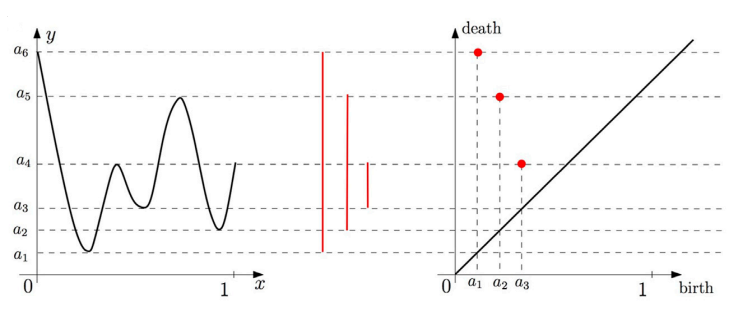
\includegraphics[width=0.85\linewidth]{./figures/Figura9.png}
    \caption{
        El c\'odigo de barras de persistencia y el diagrama de persistencia de la funci\'on
        $f:\ccorch{0,1}\rightarrow\mathbb{R}$.
    }
    \label{fig:Figura 9}
    \vspace{15pt}
\end{figure}

\section*{Ejemplo 2}

Sea $f: M\rightarrow \mathbb{R}$ la funci\'on en la Figura \ref{fig:Figura 10},
donde $M$ es una superficie de dos dimensiones homeomorfa a un toro,
y sea $F_{r} = f^{-1}\cpar{\cpar{-\infty,r}}_{r\in \mathbb{R}}$ la filtraci\'on del conjunto subnivel de $f$.
La homolog\'ia persistente cero dimensional se calcula como en el ejemplo anterior,
lo cual genera las barras rojas en el c\'odigo de barras de persistencia.
En este caso los subniveles tambi\'en almacenan informaci\'on acerca de caracter\'isticas homol\'ogicas uno dimensionales.
Cuando $r$ alcanza la altura $a_{1}$,
los conjuntos subnivel $F_{r}$ que eran homeomorfos a dos discos se vuelven homeomorfos a la uni\'on disjunta de un disco y un \'anulo,
creando un primer ciclo hom\'ologo a $\sigma_{1}$ en la Figura \ref{fig:Figura 10}.
El nacimiento de este uno-ciclo es representado por un intervalo (en azul) que comienza en $a_{1}$.
Similarmente, cuando $r$ alcanza $a_{2}$, un segundo ciclo, hom\'ologo a $\sigma_{2}$, es creado,
dando lugar al comienzo de un nuevo intervalo de persistencia.
Estos dos ciclos nunca son rellenos (abarcan $H_{1}\cpar{M}$) de manera que los intervalos que les corresponden continuan por el resto de la filtraci\'on.
Cuando $r$ alcanza $a_{3}$, un nuevo ciclo es creado, el cual se rellena en $a_{4}$,
lo cual genera el intervalo de persistencia $\cpar{a_{3},a_{4}}$.
Esta vez, la filtraci\'on del conjunto subnivel da lugar a dos c\'odigos de barras,
uno par la homolog\'ia cero dimensional (mostrado en rojo) y otro para la homolog\'ia uno dimensional (mostrado en azul).
Estos dos c\'odigos de barras pueden ser representados de manera equivalente como diagramas en el plano. 

\begin{figure}[ht]
    \centering
    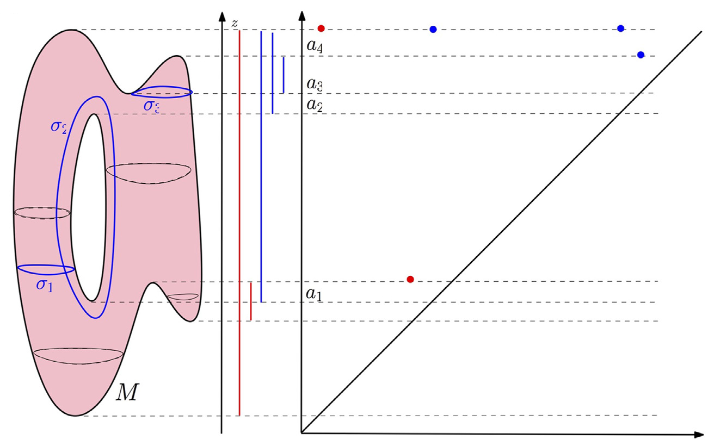
\includegraphics[width=0.85\linewidth]{./figures/Figura10.png}
    \caption{
        El c\'odigo de barras de persistencia y el diagrama de persistencia de la funci\'on altura
        (proyecci\'on en el eje $z$) definida en una superficie en $\mathbb{R}^{3}$.
    }
    \label{fig:Figura 10}
    \vspace{15pt}
\end{figure}

\section*{Ejemplo 3}

En este \'ultimo, consideramos la filtraci\'on dada por la uni\'on de bolas
(que crecen linealmente)
centradas en el conjunto de puntos finitos $C$ en la Figura \ref{fig:Figura 11}.
Notese que esta es la filtraci\'on del conjunto subnivel de la funci\'on distancia a $C$,
y gracias al teorema del nervio,
esta filtraci\'on es homot\'opicamente equivalente a la filtraci\'on de \v Cech construida sobre $C$.
La Figura \ref{fig:Figura 11} muestra varios conjuntos subnivel de la filtraci\'on de la siguiente manera:

\begin{enumerate}[label=\alph*)]
    \item Para radio $r=0$, la uni\'on de bolas se reduce al conjunto de puntos finito inicial,
    cada uno de ellos correspondiendo a una componente conexa;
    se comienza un intervalo por cada una de estas componentes en $r=0$.

    \item Algunas de las bolas comienzan a superponerse,
    resultando en la muerte de algunas de las componentes conexas que se han juntando entre s\'i;
    el diagrama de persistencia registra estas muertes, poniendo fin a los intervalos correspondientes.
    
    \item M\'as componentes conexas se han juntado, dejando una sola componente conexa,
    y as\'i, todos los intervalos asociados a caracter\'isticas cero dimensionales terminan,
    con la excepci\'on de los que corresponden a las componentes restantes;
    dos nuevas caracter\'isticas uno dimensionales han aparecido,
    lo cual resulta en dos nuevos intervalos (en azul) que comienzan en ese valor de $r$.
    
    \item Una de los dos ciclos uno dimensionales se ha rellenado,
    resultando en su muerte en la filtraci\'on y en el fin del intervalo correspondiente.
    
    \item Todas la componenetes uno dimensionales han muerto, dejando un \'unico intervalo rojo en el c\'odigo de barras.
    como en ejemplos anteriores, el c\'odigo de barras puede ser representado como un diagrama de persistencia,
    donde cada intervalo $\cpar{a,b}$ es representa por un punto en $\mathbb{R}^{2}$ de coordenadas correspondientes.
    
\end{enumerate}

Intuitivamente afirmamos que entre m\'as largo sea un intervalo en el c\'odigo de barras,
o bien, equivalentemente,
entre m\'as alejado est\'e un punto de la diagonal en el diagrama correspondiente,
m\'as persistente, y por tanto, relevante, es la propiedad homol\'ogica que le corresponde a trav\'es de la filtraci\'on.
Es de notar tambi\'en que para un radio $r$ dado, el $k$.-\'esimo n\'umero de Betti de la uni\'on de bolas en cuesti\'on,
es igual al n\'umero de intervalos de persistencia correspondiendo a caracter\'isticas homol\'ogicas $k$ dimensionales que contienen a $r$.
As\'i, el diagrama de persistencia puede ser visto como una firma topol\'ogica que codifica la homolo\'gia de la uni\'on de bolas abiertas,
para todos los radios, as\'i como su evoluci\'on a trav\'es de los valores que toma $r$.

\begin{figure}[ht]
    \centering
    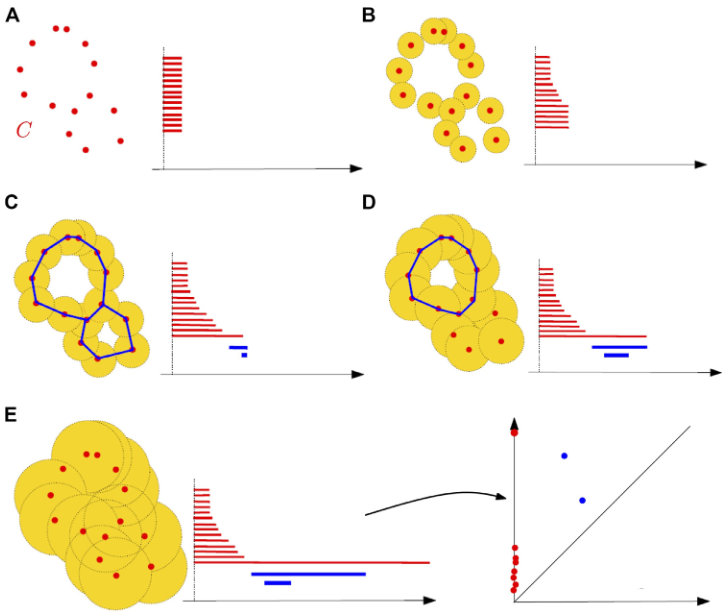
\includegraphics[width=0.85\linewidth]{./figures/Figura11.png}
    % \caption{
    %     Placeholder
    % }
    \label{fig:Figura 11}
    \vspace{15pt}
\end{figure}

\newpage

\section{M\'odulos y Diagramas de Persistencia}

Los diagramas de persistencia pueden ser formalmente definidos de manera puramente algebraica.
No obstante, lo anterior requiere de cuidado,
nos limitaremos a dar nociones b\'asicas dejando de lado sutilesas y dificultades t\'ecnicas.
Una exposici\'on detallada puede encontrarse en el trabajo por Chazal eta al. (2016)\cite{Chazal2016a}.

Sea $\mathit{Filt}=\cpar{F_{r}}_{r\in T}$ una filtraci\'on de un complejo simplicial o un espacio topol\'ogico.
Dado $K$ entero no negativo y considerando los grupos de homolog\'ia $H_{k}\cpar{F_{r}}$,
obtenemos una secuencia de espacios vectoriales donde las inclusiones $F_{r}\subset F_{r'}$, $r\leq r'$
inducen funciones lineales entre $H_{k}\cpar{F_{r}}$ y $H_{k}\cpar{F_{r'}}$.
Dicha secuencia de espacios vectoriales junto con las funciones lineales que los conectan es llamado un m\'odulo de persistencia.

\begin{definicion}
    Un m\'odulo de persistencia $\mathbb{V}$ sobre un subconjunto $T\subset\mathbb{R}$
    es una familia indexada de espacios vectoriales $\cpar{V_{r}|r\in T}$
    y una familia doblemente indexada de funciones lineales $\cpar{v_{s}^{r}:V_{r}\rightarrow V_{s}|r\leq s}$
    la cual satisface la ley de composici\'on $v_{t}^{s}\circ v_{s}^{r}=v_{t}^{r}$ donde $r\leq s\leq t$,
    y donde $v_{r}^{r}$ es la identidad en $V_{r}$.
\end{definicion}

En ocasiones, es posible descomponer un m\'odulo de persistencia en una suma directa de m\'odulos de intervalos $\mathbb{I}_{\cpar{b,d}}$ de la forma

\begin{equation*}
    \dots, \rightarrow 0 \rightarrow \dots, \rightarrow 0 \rightarrow \mathbb{Z}_{2} \rightarrow \dots, \rightarrow \mathbb{Z}_{2} \rightarrow 0 \rightarrow \dots
\end{equation*}

\noindent donde las funciones $\mathbb{Z}_{2}\rightarrow\mathbb{Z}_{2}$ son la identidad y las demas son la funci\'on $0$.
Denotando $b$ y $d$ respectivamente como el \'infimo y el supremo del intervalo de \'indices que corresponden a espacios vectoriales no cero;
dicho m\'odulo puede ser interpretado como una caracter\'istica que aparece en la filtraci\'on en el \'indice $b$ y desaparece en el \'indice $d$.
Cuando un m\'odulo de persistencia $\mathbb{V}$ puede ser descompuesto como una suma directa de m\'odulos de intervalos,
se puede mostrar que esta descomposici\'on es \'unica hasta un reordenamiento de los intervalos
(ver Chazal et al., 2016\cite{Chazal2016a}, Teorema 2.7).
Como consecuencia, el conjunto de intervalos resultantes es independiente de la descomposici\'on de $\mathbb{V}$
y es llamado el c\'odigo de barras de persistencia de $V$.
Como en los ejemplos anteriores,
cada intervalo $\cpar{b,d}$ en el codigo de barras puede ser interpretado como un punto de coordenadas $\cpar{b,d}$ en el plano $\mathbb{R}^{2}$.
La uni\'on disjunta de estos puntos, junto con la diagonal $\Delta =\cllav{x=y}$,
es un multiconjunto llamado el diagrama de persistencia de $\mathbb{V}$.

El siguiente resultado, de (Chazal et al., 2016\cite{Chazal2016a}, Teorema 2.8),
da algunas condiciones necesareas para que sea posible descomponer un m\'odulo de persistencia
en la suma directa de m\'odulos de intervalos.

\begin{teorema}
    Sea $\mathbb{V}$ un m\'odulo de persistencia con \'indices en $T\subset\mathbb{R}$.
    Si $T$ es un conjunto finito o si todos los espacios vectoriales $V_{r}$ son de dimensi\'on finita,
    entonces $\mathbb{V}$ se puede descomponer en una suma directa de m\'odulos de intervalos.
    M\'as a\'un, para cualquier $s,\hspace{2pt}t\in T$, $s\leq t$,
    el n\'umero $\beta_{t}^{s}$ de intervalos que inician antes antes que $s$ y finalizan despues que $t$
    es igual al rango de la funci\'on lineal $v_{t}^{s}$
    y es llamado el n\'umero de Betti \linebreak $\cpar{s, t}$-persistente de la filtraci\'on.
\end{teorema}

Debido a que se satisfacen ambas de las condiciones anteriores para la homolog\'ia persistente de filtraciones de complejos simpliciales finitos,
una consecuencia inmediata de este resultado es que los diagramas de persistencia de dichas filtraciones siempre est\'an bien definidos.

As\'i, es posible mostrar que los diagramas de persistencia pueden ser definidos tan pronto como la siguiente condicion se satisfaga.

\begin{definicion}
    Un m\'odulo de $\mathbb{V}$ con \'indices en $T\subset\mathbb{R}$ es $q$-d\'ocil
    si para todo $r<s$ en $T$, el rango de la funci\'on lineal $v_{s}^{r}:V_{r}\rightarrow V_{s}$ es finito.
\end{definicion}

\begin{teorema}
    Chazal et al. (2009)\cite{Chazal2009a}, Chazal et al. (2016)\cite{Chazal2016a}.
    Si $\mathbb{V}$ es un m\'odulo de persistencia $q$-d\'ocil,
    entonces tiene un diagrama de persistencia bien definido.
    Dicho diagrama de persistencia $\mathrm{dgm}\cpar{\mathbb{V}}$
    es la uni\'on de los puntos de la dioagonal $\Delta$ de $\mathbb{R}^{2}$,
    contados con multiplicidad infinita,
    y un multiconjunto sobre la diagonal en $\mathbb{R}^{2}$ que es localmente finito.
    Aqu\'i, con localmente finito nos referimos a que
    para cualquier rect\'angulo $R$ con lados paralelos a los ejes coordenados que no intersecan a $\delta$,
    el n\'umero de puntos de $\mathrm{dgm}\cpar{\mathbb{V}}$, contados con multiplicidad,
    contenidos en $R$ es finito.
    Adem\'as, a la parte del diagrama hecha de los puntos con segunda coordenada infinita
    es llamada la parte escencial del diagrama.
\end{teorema}

La construcci\'on de diagramas de persitencia para m\'odulos $q$-d\'ociles
esta fuera de nuestro margen de estudio,
pero da lugar a las mismas nociones que en el caso de m\'odulos descomponibles.
Puede ser creados siguiendo el acercamiento algebraico
basado en las propiedades de descomposibilidad de los m\'odulos
o adoptando un acercamento por el lado de la teor\'ia de la medida,
la cual nos permite definir diagramas como medidas con valores enteros en un espacio de rect\'angulos en el plano.
Vease Chazal et al. (2016)\cite{Chazal2016a} para m\'as informaci\'on.

Aunque los m\'odulos de persistencia encontrados en la pr\'actica son descomponibles,
la estructura general de los m\'odulos de persistencia $q$-d\'ociles juega un papel fundamental
en el an\'alisis matem\'atico y estad\'istico de la homolog\'ia persistente.
En especial al momento de asegurar la existencia de los diagramas l\'imite
cuando se estudian propiedades de convergencia (Ver Cap\'itulo \ref{chap:Cap5}).

Una filtraci\'on $\mathrm{Filt}=\cpar{F_{r}}_{r\in T}$ de un complejo simplicial
o un espacio topol\'ogico es llamado d\'ocil si para cualquier entero $k$,
el m\'odulo de persistencia $\cpar{H_{k}\cpar{F_{r}}|r\in T}$ es $q$-d\'ocil.
Es de notar que las filtraciones de complejos simpliciales finitos siempre son dociles.
Como consecuencia de lo anterior, para cualquier entero $k$,
el diagrama de persistencia denotado $\mathrm{dgm}_{k}\cpar{\mathrm{Filt}}$
es asociado con la filtraci\'on $\mathrm{Filt}$.
Cuando $k$ no se especifica de manera expl\'icita y no hay ambig\"uedadm
es com\'un dejar fuera de la notaci\'on el \'indice $k$ y hablar de ``el''
diagrama de persistencia $\mathrm{dgm}\cpar{\mathrm{Filt}}$ de la filtraci\'on $\mathrm{Filt}$.
Esta notaci\'on se entiende como
``$\mathrm{dgm}_{k}\cpar{\mathrm{Filt}}$ para alguna $k$.''

\section{Paisajes de persistencia}

Los paisajes de persistencia introducidos en Bubenik (2015) \cite{Bubenik2015}
es una representaci\'on alternativa de los diagrama de persistencia.
Este acercamiento se enfoca en representa la informaci\'on topol\'ogica
codificada en los diagramas de persitencia como elementos de un espacio de Hilbert,
en el cual m\'etodos de aprendizaje estad\'istico pueden ser directamente aplicados.
Los paisajes de persistencia son una colecci\'on de funciones continuas y lineales
por pedazos $\lambda:\mathbb{N}\times\mathbb{R}\rightarrow\mathbb{R}$
las cuales resumen un diagrama de persistencia $\mathrm{dgm}$.

Un par $p=\cpar{b,d}\in\mathrm{dgm}$ es transformado en el punto
$\cpar{\frac{b+d}{2},\frac{d-b}{2}}$ (Ver Figura \ref{fig:Figura 12}).
En esta definici\'on descartamos los puntos con persistencia infinita.
El paisaje se define entonces considerando el conjunto de funciones creadas
cubriendo las caracter\'isticas del diagrama de persistencia rotado como sigue:

\begin{equation*}
    \Lambda_{p}\cpar{t} =
    \begin{cases*}
        t-b & $t\in\ccorch{b,\frac{b+d}{2}}$ \\
        d-t & $t\in\left(\frac{b+d}{2},d\right]$ \\
        0 & en otro caso.
    \end{cases*}
\end{equation*}

El paisaje de persistencia $\lambda_{\mathrm{dgm}}$ de $\mathrm{dgm}$ es un resumen
del arreglo de curvas lineales por pedazos que se obtiene al sobreponer las gr\'aficas
de las funciones $\cllav{\Lambda_{p}}_{p\in\mathrm{dgm}}$.
Formalmente, el paisaje de persistencia de $\mathrm{dgm}$ es una colecci\'on de funciones

\begin{equation*}
    \lambda_{\mathrm{dgm}}\cpar{k,t} =
    \underset{r\in\mathrm{dgm}}{\mathrm{kmax}}\text{ }\Lambda_{r}\cpar{t},
    \text{  }t\in\ccorch{0,T},k\in\mathbb{N},
\end{equation*}

\noindent donde $\mathrm{kmax}$ es el $k$-\'esimo valor m\'as grande del conjunto.
Dado $k\in\mathbb{N}$, la funci\'on $\lambda_{dgm}\cpar{k,.}:\mathbb{R}\rightarrow\mathbb{R}$
es llamado el $k$-\'esimo paisaje de persistencia de $\mathrm{dgm}$.
M\'as a\'un, una funci\'on que asocia cada diagrama de persistencia con su paisaje correspondiente
es inyectiva.
En otras palabras, no se pierde inforamci\'on cuando se utiliza un paisaje de persistencia
para representar un diagrama.

\begin{figure}[ht]
    \centering
    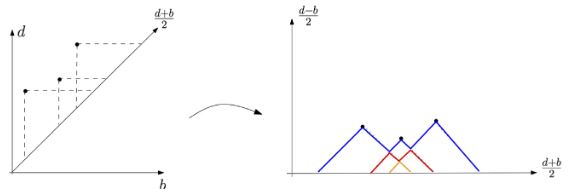
\includegraphics[width=0.85\linewidth]{./figures/Figura12.JPG}
    \caption{
        Ejemplo de un paisaje de persitencia (derecha) asociado con un
        diagrama de persistencia (izquierda).
    }
    \label{fig:Figura 12}
    \vspace{15pt}
\end{figure}

La ventajas de la representaci\'on por paisajes de persistencia son.
Primero, los diagramas de persistencia se convierten en elementos de un espacio funcional,
permitiendo el uso de una variedad m\'as amplia de herramientas de la estad\'istica y
el an\'alisis de datos para el procesamiento de character\'isticas topol\'ogicas,
vease Bubenik (2015)\cite{Bubenik2015}, Chazal et al. (2015)\cite{Chazal2014b}.
Segundo, y fundamental para la perspectiva te\'orica,
los paisajes de persistencia comparten las mismas propiedades de estabilidad
que los diagramas de persistencia (Ver Secci\'on \ref{sec: 4.7}).

\section{Representaciones Lineales de la Persistencia Homol\'ogica}

Un diagrama de persistencia sin su parte escencial puede representarse como
una medida discreta $\delta^{+}=\cllav{p=\cpar{b,d},b<d<\infty}$.
Con un ligero abuso de la notaci\'on, podemos escribir lo siguiente:

\begin{equation*}
    \mathrm{dgm}=\sum_{p\in\mathrm{dgm}}\delta_{p},
\end{equation*}

\noindent donde las caracter\'isticas son contadas con multiplicidad y
$\delta_{\cpar{b,d}}$ denota la medida de Dirac en $p=\cpar{b,d}$.
La mayoria de los descriptores propuestos para analizar la persistencia pueden
ser expresados como transformaciones lineales de un diagrama de persistencia,
vistos como:

\begin{equation*}
    \Psi\cpar{\mathrm{dgm}}=\sum_{p\in\mathrm{dgm}}f\cpar{p},
\end{equation*}

\noindent para alguna funci\'on $f$ definida en $\Delta$ que toma valores en
un espacio de Banach.

En la mayoria de los casos, queremos que estas transformaciones se apliquen de manera
independiente a cada dimensi\'on homol\'ogica. Para $k\in\mathbb{N}$ alguna dimensi\'on
homol\'ogica dada, consideramos alguna transformaci\'on lineal del diagrama de persistencia
restringida a las caracter\'isticas topol\'ogicas de la dimensi\'on $k$ como sigue:

\begin{equation}\label{eq: 4.5}
    \Psi_{k}\cpar{\mathrm{dgm}_{k}}=\sum_{p\in\mathrm{dgm}_{k}}f_{k}\cpar{p},
\end{equation}

\noindent donde $\mathrm{dgm}_{k}$ es el diagrama de persistencia de las caracter\'isticas
topol\'ogicas de la dimensi\'on $k$ donde $f_{k}$ est\'a definido en $\Delta$ y toma valores
en un espacio de Banach.

\section*{Curvas de Betti}

La manera m\'as sencilla de representar la persistencia homol\'ogica es la funci\'n
de Betti o curva de Betti. La curva de Betti de una dimensi\'on homol\'ogica $k$ esta
definida como:

\begin{equation*}
    \beta_{k}\cpar{t}=\sum_{\cpar{b,d}\in\mathrm{dgm}}w\cpar{b,d}\mathds{1}_{t\in\ccorch{b,d}}
\end{equation*}

\noindent donde $w$ es una funci\'on peso definida en $\Delta$. En otras palabras,
la curva de Betti es el n\'umero de cadigos de barra en el tiempo $m$.
Este descriptor es una reapresentaci\'on linear de la homolog\'ia persistente,
tomando $f$ como en (\ref{eq: 4.5}) de forma que
$f\cpar{b,d}\cpar{t}=w\cpar{b,d}\mathds{1}_{t\in\ccorch{bd}}$.
Una elecci\'on t\'ipica para la funci\'on peso es una funci\'on creciente de la persistencia
$w\cpar{b,d}=\tilde{w}\cpar{d-b}$ donde $\tilde{w}$ es una funci\'on creciente definida en $\mathbb{R}^{+}$.
Una de las primeras aplicaciones de las curvas de Betti se puede encontrar en Umeda (2017)\cite{Umeda2017}.

\section*{Superficies de Persistencia}

Una superficie de persistencia (tambi\'en llamadas im\'agenes de persistencia)
se obtiene mediante la convoluci\'on de un diagrama de persistencia con un kernel.
Introducidas en Adams et al. (2017)\cite{Adams2017}. Sea $K:\mathbb{R}^{2}\rightarrow\mathbb{R}$,
un kernel, y $H$ una matriz $2\times 2$ sim\'etrica y definida positiva,
y dada $u\in\mathbb{R}^{2}$ definimos

\begin{equation*}
    K_{H}\cpar{u}=\det\cpar{H}^{-\frac{1}{2}}K\cpar{H^{-\frac{1}{2}}u}.
\end{equation*}

Sea $w:\mathbb{R}^{2}\rightarrow\mathbb{R}_{+}$ una funci\'on peso definida en $\Delta$.
Se define la superficie de persistencia homol\'ogica de dimensi\'on $k$ asociada con el diagrama $\mathrm{dgm}$,
con kernel $K$ y matriz $H$ como sigue:

\begin{equation*}
    \forall u\in\mathbb{R}^{2},
    \rho_{k}\cpar{\mathrm{dgm}}\cpar{u}=
    \sum_{p\in\mathrm{dgm}_{k}}w\cpar{r}K_{H}\cpar{u-p}
\end{equation*}

La superficie de persistencia es entonces una represetaci\'on lineal de la persistencia homol\'ogica.
T\'ipicamente las funciones peso son funciones crecientes de la persistencia.

\section{M\'etricas en el Espacio de Diagramas de Persistencia}
Para aprovechar la informaci\'on y caracter\'isticas topol\'ogicas inferidas por la
homologi\'ia persistente, necesitamos alguna manera de comparar diagramas de persistencia,
esto es, otorgar al espacio de los diagramas de persistencia una estructura de espacio m\'etrico.
Aunque se han considerado una variedad de m\'etricas, la m\'as fundamental de ellas se le conoce como
la distancia de cuello de botella.

\begin{figure}[ht]
    \centering
    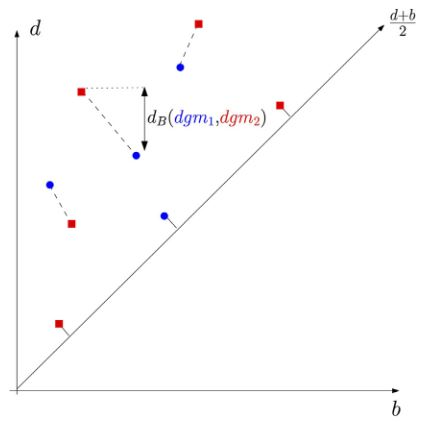
\includegraphics[width=0.85\linewidth]{./figures/Figura13.JPG}
    \caption{
        Emparejamiento perfecto y la distancia de cuello de botella entre un
        diagrama en rojo y un diagrama en azul. N\'otese que algunos puntos
        en ambos diagramas son emparejados a puntos en la diagonal.
    }
    \label{fig:Figura 13}
    \vspace{15pt}
\end{figure}

Recordemos que un diagrama de persistencia es la uni\'on de un multiconjunto discreto
en la parte del plano por encima de la diagonal $\Delta$ y,
por razones t\'ecnicas que veremos adelante,
$\Delta$, donde el punto de $\Delta$ se cuenta con multiplicidad infinita.
Un emparejamiento (ver Figura \ref{fig:Figura 13}) entre dos diagramas,
$\mathrm{dgm}_{1}$ y $\mathrm{dgm}_{2}$, es un subconjunto
$m\subseteq\mathrm{dgm}_{1}\times\mathrm{dgm}_{2}$ tal que cada punto en
$\mathrm{dgm}_{1} - \Delta$ y $\mathrm{dgm}_{2} - \Delta$ aparece exactamente
una vez en $m$.
En otras palabras, para cada $p\in\mathrm{dgm}_{1} - \Delta$ y para cualquier
$q\in\mathrm{dgm}_{2} - \Delta$, $\cpar{\cllav{p}\times\mathrm{dgm}_{2}}\cap m$
y $\cpar{\mathrm{dgm}_{1}\times\cllav{q}}\cap m$ contiene cada uno un \'unico par.
La distancia de cuello de botella entre $\mathrm{dgm}_{1}$ y $\mathrm{dgm}_{2}$
esta definida como

\begin{equation*}
    \mathrm{d}_{\mathrm{b}}\cpar{\mathrm{dgm}_{1},\mathrm{dgm}_{2}} =
    \inf_{\text{empar. }m}\max_{\cpar{p,q}\in m}\cnorm{p-q}_{\infty}.
\end{equation*}

El c\'alculo pr\'actico de la distancia de cuella de botella se resume en
encontrar un cierto emparejamiento perfecto en gr\'aficas bipartitas, y para esto
podemos utilizar algoritmos cl\'asicos.

La distancia de cuello de botella es una m\'etrica parecida a una m\'etrica $\mathit{L}_{\infty}$.
Resulta ser una m\'etrica natural para expresar las propiedades de estabilidad de los
diagramas de persistencia presentados en la secci\'on \ref{sec: 4.7},
pero sufre de las mismas desventajas que las m\'etricas usuales en $\mathit{L}_{\infty}$,
esta completamente determinada por la mayor distancia entre los pares
y no toma en cuenta la cercania de los pares de puntos restantes.
Una variante para superar este problema, es la distancia de Wasserstein entre diagramas.
Dada $p\geq 1$, se define como

\begin{equation*}
    \mathrm{W}_{p}\cpar{\mathrm{dgm}_{1},\mathrm{dgm}_{2}}^{p} =
    \inf_{\text{empar. }m}\sum_{\cpar{p,q}\in m}\cnorm{p-q}_{\infty}^{p}
\end{equation*}

Se han presentado resultados de utilidad acerca de la persistencia en la m\'etrica $\mathrm{W}_{p}$,
particularmente en el estudio por Cohen-Steiner et al. (2010)\cite{Cohen2010},
pero dependen de supuestos que los vuelve consecuencias de los resultados de estabilidad
en la distancia de cuello de botella.
Un estudia general del espacio de diagramas de persistencia dotado con m\'etricas
$\mathrm{W}_{p}$ se ha considerada en Divol y Lacombe (2020)\cite{Divol2021},
donde so propone un marco general basado en transportes parciales \'optimos,
donde muchas propiedades importantes de los diagramas de persistencia pueden probarse de manera natural.

\section{Propiedades de Estabilidad en los Diagramas de Persistencia}\label{sec: 4.7}

Una propiedad fundamental de la homolog\'ia persistente es que
los diagramas de persistencia de filtraciones construidas sobre conjuntos de datos
resultan ser muy estables con respecto a ciertas perturbaciones de los datos.
Para formalizar y cuantificar dichas propiedades, primero necesitamos ser precisos
con respecto a que perturbaciones son permitidas.

En lugar de trabajar directamente con filtraciones sobre conjuntos de datos,
resulta ser m\'as conveniente definir una noci\'on de proximidad entre m\'odulos
de persistencia, de donde derivaremos un resultado de estabilidad general para la
homolog\'ia persistente. Entonces, la mayoria de los resultados de estabilidad
para filtraciones especificas ser\'an consecuencia de este teorema general.
Para evitar discuciones t\'ecnicas y sin p\'erdida de generalidad, suponemos
que los m\'odulos de persistencia considerados est\'an indexados por $\mathbb{R}$.

\begin{definicion}
    Sean $\mathbb{B}$, $\mathbb{W}$ dos m\'odulos de persistencia indexados por
    $\mathbb{R}$. Dado $\delta\in\mathbb{R}$, un homomorfismo de grado $\delta$ entre
    $\mathbb{V}$ y $\mathbb{W}$ es una colecci\'on $\Phi$ de funciones lineales
    $\phi_{r}:V_{r}\rightarrow W_{r+\delta}$, para todo $r\in\mathbb{R}$ tal que
    para cualquier $r\leq s$, $\phi_{r}\circ v_{s}^{r}=w_{s+\delta}^{r+\delta}\circ\phi_{r}$.
\end{definicion}

Un ejemplo importante de un homomorfismo de grado $\delta$ es el endomorfismo de cambio
$\mathrm{1}_{\mathbb{V}}^{\delta}$ el cual consiste de las familias de funciones lineales
$\cpar{v_{r+\delta}^{r}}$. N\'otese que los homomorfismos de m\'odulos pueden ser
naturalmente compuestos; la compisici\'on de un homomorfismo $\Psi$ de grado $\delta$
entre $\mathbb{U}$ y $\mathbb{V}$ y un homomorfismo $\Phi$ de grado $\delta'$ entre
$\mathbb{V}$ y $\mathbb{W}$ naturalmente da lugar a un homomorfismo $\Phi\Psi$ de
grado $\delta + \delta'$ entre $\mathbb{U}$ y $\mathbb{W}$.

\begin{definicion}
    Sea $\delta\geq 0$. Dos m\'odulos de persistencia $\mathbb{V}$, $\mathbb{W}$
    son $delta$-intercalados si existen dos homomorfismos de grado $\delta$,
    $\Phi$, de $\mathbb{V}$ a $\mathbb{W}$ y $\Psi$ de $\mathbb{W}$ a $\mathbb{V}$
    tales que $\Psi\Phi = \mathrm{1}_{\mathbb{V}}^{2\delta}$ y
    $\Phi\Psi = \mathrm{1}_{\mathbb{W}}^{2\delta}$.
\end{definicion}

Aunque no define un am\'etrica en el espacio de los m\'odulos de persistencia,
la noci\'on de cercania entre dos m\'odulos de persistencia puede ser definida como
el m\'as peque\~{n}o $\delta$ no negativo tal que los m\'odulos sean $\delta$-intercalados.
M\'as a\'un, nos ayuda a formalizar el siguiente teorema fundamental
(Chazal et al., 2009\cite{Chazal2009a}; Chazal et al., 2016\cite{Chazal2016a}).

\begin{teorema}[Estabilidad de la persistencia]\label{teo:EstPersist}
    Sean $\mathbb{V}$ y $\mathbb{W}$ dos m\'odulos de persistencia $q$-d\'ociles.
    Si $\mathbb{V}$ y $\mathbb{W}$ son $\delta$-intercalados para alg\'un $\delta>0$,
    entonces
    \begin{equation*}
        \mathrm{d}_{\mathrm{b}}
        \cpar{\mathrm{dgm}\cpar{\mathbb{V}},\mathrm{dgm}\cpar{\mathbb{W}}}\leq\delta.
    \end{equation*}
\end{teorema}

Con este resultado obtenemos una herramienta eficiente para establecer resultados de
estabilidad concretos en el ATD. Por ejemplo, podemos recuperar el primer resultado de
estabilidad de la persistencia que aparece en la literatura
(Cohen-Steiner et al., 2005)\cite{Cohen2005}.

\begin{teorema}
    Sean $f,g:M\rightarrow\mathbb{R}$ dos funciones de valores reales definidas en un
    espacio topol\'ogico $M$ que son $q$-d\'ociles, esto es, que sus filtraciones de
    los conjuntos subnivel de $f$ y $g$ inducen m\'odulos $q$-d\'ociles en el nivel de
    la homolog\'ia. Entonces, para cualquier entero $k$,
    \begin{equation*}
        \mathrm{d}_{\mathrm{b}}
        \cpar{\mathrm{dgm}_{k}\cpar{f},\mathrm{dgm}_{k}\cpar{g}}\leq
        \cnorm{f-g}_{\infty}=
        \sup_{x\in M}\cabs{f\cpar{x}-f\cpar{x}}
    \end{equation*}
    donde $\mathrm{dgm}_{k}\cpar{f}$ es el diagrama de persistencia de el m\'odulo
    de persistencia $\cpar{H_{k}}\cpar{f^{-1}\cpar{-\infty,r}}|r\in\mathbb{R}$,
    y respectivamente para $\mathrm{dgm}_{k}\cpar{f}$,
    donde las funciones lineales son las inducidas por las inclusiones can\'onicas
    entre los conjuntos subnivel.
\end{teorema}
\begin{prueba}
    Denotamos $\delta=\cnorm{f-g_{\infty}}$, tenemos que para cualquier $r\in\mathbb{R}$,
    $f^{-1}\cpar{-\infty,r}\subseteq g^{-1}\cpar{-\infty,r+\delta}$ y
    $g^{-1}\cpar{-\infty,r}\subseteq f^{-1}\cpar{-\infty,r+\delta}$.
    este intercalado entre los conjuntos subnivel de f induce un $\delta$-intercalamiento
    entre los m\'odulos de persistencia en el nivel de la homolog\'ia,
    y as\'i, el resultado se sigue de una aplicaci\'on directa del teorema anterior.
\end{prueba}

El \emph{Teorema \ref{teo:EstPersist}} tambi\'en implica el siguiente resultado
de estabilidad para los diagramas de persistencia de filtraciones construidas sobre
conjuntos de datos.

\begin{teorema}
    Sean $\mathbb{X}$ y $\mathbb{Y}$ dos espacios m\'etricos compactos y sean
    $\mathrm{Filt}\cpar{\mathbb{X}}$ y $\mathrm{Filt}\cpar{\mathbb{Y}}$ las
    filtraciones de Vietoris-Rips o de \v Cech contruidos sobre $\mathbb{X}$ y
    $\mathbb{Y}$. Entonces
    \begin{equation*}
        \mathrm{d}_{\mathrm{b}}
        \cpar{\mathrm{dgm}\cpar{\mathrm{Filt}\cpar{\mathbb{X}}},
        \mathrm{dgm}\cpar{\mathrm{Filt}\cpar{\mathbb{Y}}}}\leq
        2\mathrm{d}_{\mathrm{GH}}\cpar{\mathbb{X},\mathbb{Y}}
    \end{equation*}
    donde $\mathrm{dgm}\cpar{\mathrm{Filt}\cpar{\mathbb{X}}}$ y
    $\mathrm{dgm}\cpar{\mathrm{Filt}\cpar{\mathbb{Y}}}$ denotan los
    diagramas de persistencia de las filtraciones $\mathrm{Filt}\cpar{\mathbb{X}}$ y
    $\mathrm{Filt}\cpar{\mathbb{Y}}$.
\end{teorema}